\documentclass[10pt,twocolumn]{article} 
\usepackage{simpleConference}
\usepackage{times}
\usepackage{graphicx}
\usepackage{amssymb}
\usepackage{url,hyperref}
\usepackage{amsmath}
\usepackage{multirow}
\usepackage{rotating}

\setlength{\rotFPtop}{0pt plus 1fil}

%caption loading 
\usepackage{caption3}
\DeclareCaptionOption{parskip}[]{} 
\usepackage[small]{caption}

\begin{document}

\title{Examining Phylogenetic Reconstruction Algorithms}

\author{
Evan Albright\\
\texttt{ichbinevan@gmail.com}
\and
Jack Hessel\\
\texttt{jmhessel@gmail.com}
\and
Nao Hiranuma\\
\texttt{hiranumn@gmail.com}
\and
Cody Wang\\
\texttt{mcdy143@gmail.com}
}

\maketitle
\thispagestyle{empty}

\begin{abstract}
Understanding the evolutionary relationships between organisms by comparing their genomic sequences
is a focus of modern-day computational biology research. Estimating evolutionary history in this way 
has many applications, particularly in analyzing
the progression of infectious, viral diseases. Phylogenetic reconstruction algorithms model
evolutionary history using tree-like structures that describe the estimated ancestry of a given set
of species. Many methods exist to infer phylogenies from genes, but no one technique is
definitively better for all types of sequences and organisms. Here, we implement and analyze
several popular tree reconstruction methods and compare their effectiveness on both synthetic
and real genomic sequences. Our synthetic data set aims to simulate a variety of research
conditions, and includes inputs that vary in number of species. For our case-study, we use the genes of 53 apes and compare our reconstructions
against the well-studied evolutionary history of primates. Though our implementations often
represent the simplest manifestations of these complex methods, our results are suggestive of
fundamental advantages and disadvantages that underlie each of these techniques.
\end{abstract}

\section*{Introduction}
\subsection*{Phylogenetic Trees}
A phylogenetic tree, commonly referred as a tree of life, is a widely accepted representation of evolutionary relationship among species on the Earth \cite{Baum-Phylotree}. The concept of a tree of life was first introduced by Charles Darwin in 1836 after his trip to Galapagos islands (Figure \ref{darwintree}). Each node in a tree is called a taxonomic unit, or ``taxa,'' for short. Internal nodes in a tree represent most common ancestors of their direct child nodes. The length of a branch in a phylogenetic tree is an indication of evolutionary distance. Depending on the particular reconstruction method used, branch length usually indicates either the estimated time it took for one species to evolve into another species, or the genetic distance between a pair of an ancestor and its descendant. We are particularly interested in bifurcating phylogenetic trees, meaning an ancestor can only have two direct descendants.

Phylogenetic trees are useful not only for describing the evolutionary history of multiple species but also for solving other real world problems. For instance, phylogenetic analysis of a virus can sometime help us track down the source of infectious, viral diseases such as SARS \cite{li2005bats}. Phylogenetic trees are also used to find natural sources of new drugs or to develop effective treatments against diseases that are hard to cure \cite{Pillai-HIV}. Reconstruction also allows us to make predictions about poorly understood or extinct species. All these applications are dependent on our ability to reconstruct phylogenetic trees from information available to us. 

Here, we implement, apply, and compare several popular multiple sequence alignment algorithms (MSAs) and phylogenetic reconstruction methods. Because these algorithms are so commonly applied, state-of-the-art implementations for each exist. We acknowledge our programs lack the nuance and optimizations found in these refined and expert versions. However, we argue that results derived from our bare-bones implementations reflect basic advantages and disadvantages that underlie each method.

\begin{figure}[ht!]
\centering
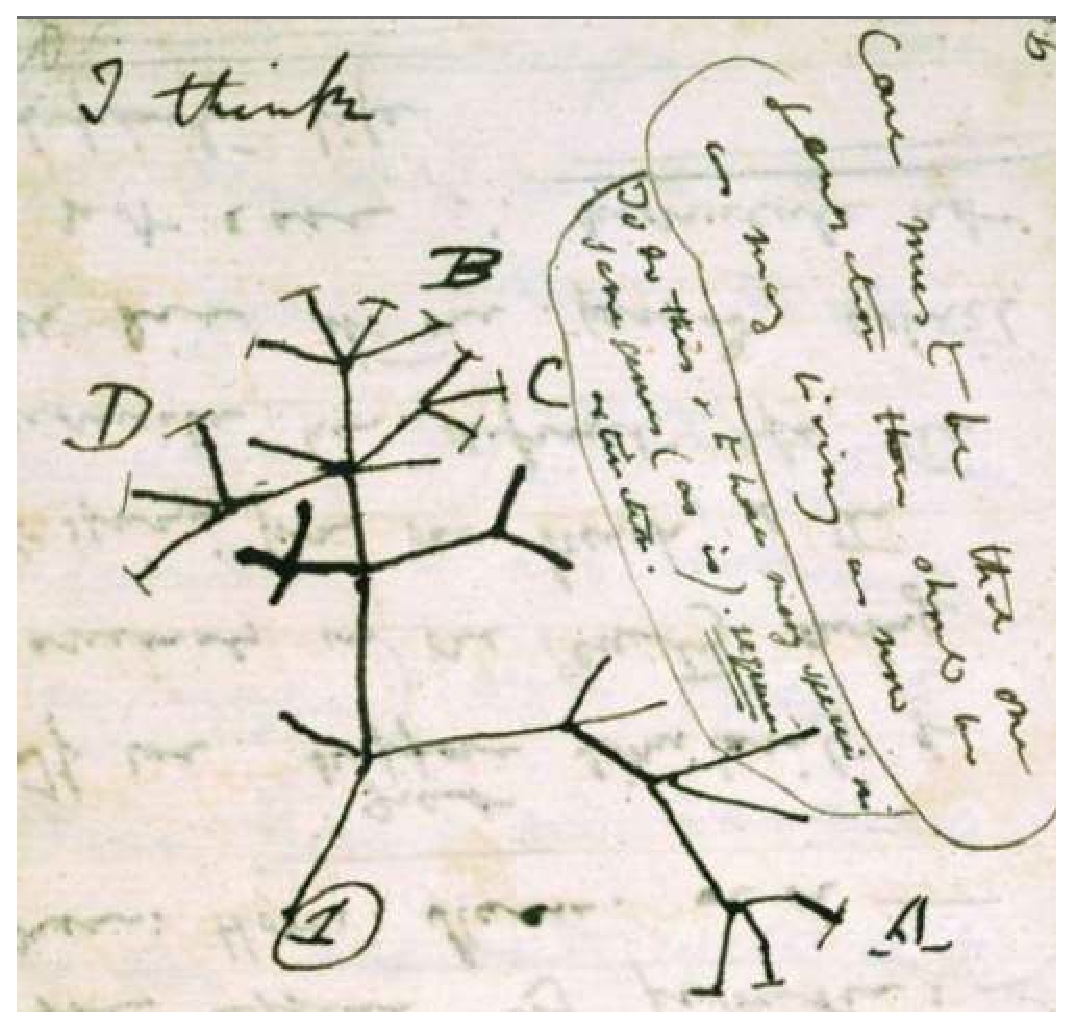
\includegraphics[width=80mm]{media/ithink.eps}
\caption{The first phylogenetic tree drawn by Charles Darwin on his notebook on mid-July, 1837.}
\label{darwintree}
\end{figure}

All phylogenetic algorithms examined by our group can be labeled as ``cladistics.'' Cladistic methods attempt to identify relationships based on shared, inherited characteristics amongst individuals. Cladisitcs group organisms using similarities derived from common ancestors and splitting events, with evolutionary history in mind. In contrast to cladistic methods, ``phenetic'' methods shift their emphasis to morphological similarities independent of ancestry. Generally, phenetic methods are not considered to be state-of-the-art and we do not consider them further here.

For our study, we execute our algorithms on both synthetic data and real-world genetic sequences. Synthetic data is useful because the underlying evolutionary history can be known completely. We implement a data generator that creates a random, but exactly determined, phylogenetic tree, and outputs genomic sequences that might be produced given that tree as the true evolutionary history.

Due to a lack of commonly agreed upon historical data, it is usually impossible to determine whether or not a constructed phylogenetic tree is accurate when using actual genomic sequences. One of the few areas within phylogenetics wherein experts generally agree is the evolutionary history is apes. We choose to use apes as our study case to examine algorithmic performance because there exists a commonly accepted baseline to compare our results against.

Phylogenetics is a field with significant nuances and complexity. For instance, there are multiple issues confounding tree construction: chiefly homoplasy, whereby some nucleic characters are likelier to evolve convergently, and horiztonal gene transfer, whereby genes may be transferred outside the parent-child relationship. Because each of our bare-bones implementations makes simplifying assumptions that ignore these complexities, applying these methods to real genes might help us assess their sensitivity to these uncontrolled for processes.

\subsection*{Project Goals}
There is no single best algorithm in phylogenetic reconstruction. It's possible to produce pathological cases where certain algorithms perform better than others, and there exists substantial variability in potential inputs, depending on the specific organisms to be evaluated. Furthermore, exploration is too costly with large numbers of lengthy sequences for exhaustive search to be feasible. To explore an entire set of possible topologies, for instance, a problem with $n$ input species would require $(2n-5)!/[(n-3)! 2^{n-3}]$ constructions \cite{heywood1964phenetic}. Thus, it is our goal to explore the contexts in which our algorithms are most effective, analyzing their efficiency and efficacy in producing a tree of relationships amongst a set of taxa.

After conducting a literature review and determining which types of algorithms were
most frequently utilized, we decided to implement the following six phylogenetic reconstruction
algorithms, three multiple sequence alignment algorithms, and two tree comparison methods.


\begin{itemize}
\item Multiple Sequence Alignments:
  \begin{itemize}
    \item \textbf{Clustal-W (CW)}\\
      A progressive alignment method which computes a ``guide tree'' based on possible all pairwise
      sequence alignments. The guide tree is then collapsed to produce the final multiple sequence
      alignment.
    \item \textbf{MUSCLE (MSC)}\\
      An iterative alignment method similar to Clustal-W that foregoes computing initial
      pairwise alignments in favor of later iterative improvement. 
    \item \textbf{Center Star (CS)}\\
     A simplistic alignment method that identifies the ``center" sequence which all other sequences are aligned to. 
     The pairs of the center and every other sequence are combined into the final multiple alignment.
  \end{itemize}
\item Tree Reconstruction Algorithms:
  \begin{itemize}
    \item \textbf{Neighbor-joining (NJ)}\\
      A distance matrix method that attempts to reconstruct a tree through an agglomerative
      clustering approach.
    \item \textbf{Maximum Likelihood (ML) with hill-climbing and progressive topology searches}\\
      A method which uses known mutation rates between nucleotides to
      recursively evaluate the ``likelihood'' of a given tree. We use the principle
      of ML to produce a final tree using two topology search heuristics, ``hill-climbing''
      and ``progressive'' (referred to as MLH and MLP, respectively).
    \item \textbf{Maximum Parsimony (MP) with hill-climbing and progressive topology searches}\\
      An evaluation based in the concept of parsimony, wherein trees with the least
      mutation required to group taxa are highly valued. We use the principle
      of MP to produce a final tree using two topology search heuristics, ``hill-climbing''
      and ``progressive'' (referred to as MPH and MPP, respectively).
    \item \textbf{Monte-Carlo Markov Chain (MCMC or MC)}\\
      An implementation of the Metropolis-Hastings algorithm which allows us to sample
      from a distribution of the most likely evolutionary trees.
  \end{itemize}
\item Tree Comparison Metrics:
  \begin{itemize}
    \item \textbf{Pairwise Pathlength Distance (PPLD)}\\
      A distance metric that relies on the distances between
      all pairs of species in a given tree. 
    \item \textbf{Quartet Distance (QD)}\\
      A distance metric that measures the topological distance between
      input trees using quartet reductions.
  \end{itemize}
\end{itemize}

A total phylogenetic reconstruction consists of a sequence alignment step
followed by a tree reconstruction step. In total, we have 18 possible
phylogenetic reconstruction methods, given our three sequence aligners and our six tree reconstructors.

Previous studies of the relative efficiencies and correctness of these
algorithms are extensive but inconsistent. Most studies reach a consensus
that distance-matrix based algorithms (i.e. NJ) generally outperform
MP in both correctness and efficiency, regardless of nucleotide substitution
rates. This is because of MP only uses sequence information from
informative sites, and because it cannot adjust for multiple mutations \cite{sourdis1988relative}. Other studies claim that with uniform rates of evolution among branches, distance methods are inferior to parsimony both with short sequences with low rates ($\sim 0.01$) and with long sequences with high rates ($\sim 0.1$), and were slightly superior in the other cases \cite{kuhner1994simulation}.

In comparing NJ and ML methods, study results also vary. Saito, Naruya, and 
Imanishi maintain that when constant rates of nucleotide substitution 
rates among sites are assumed, the NJ method showed slightly better
performance than ML, but inferior to ML when substitution rates varied
drastically \cite{saitou1989relative}. In contrast, Hasegawa, Masami, and
Fujiwara find that NJ is also robust to heterogeneity of evolutionary rates
among sites given that heterogeneity is considered in estimating the
multiple-hit effect \cite{hasegawa1993relative}. 

In comparing estimations of tree branch lengths, previous work suggests that when a low nucleotide substitution rates ($\sim 0.01$) is assumed, NJ, MP, and ML are equally successful, while for higher rates ($\sim 0.1$), ML is slightly better \cite{kuhner1994simulation}.

Markov Chain Monte Carlo (MCMC) methods are useful when an estimate of the posterior distribution of phylogenetic trees under specific prior assumptions is desired \cite{salter2000algorithms}. Methods utilizing MCMC are easily extended to Bayesian analysis, and, consequently, tree reconstructions using this algorithm are often phrased in that context. Compared with NJ, MP, and ML methods, MCMC has the advantage of being able to create a distribution of trees and constructing a ``confidence set.'' In addition, this distribution of trees can be used to study the variability in any aspect of the phylogeny that is of interest. For instance, if you were interested in computing the variability in total tree diameter, MCMC could provide draws from an entire tree distribution to compute statistics and confidence intervals from. However, it gives poor estimates of the posterior probability of any individual tree when the number of taxa is large \cite{salter2000algorithms}. 

In terms of computational time, Saito, Naruya, and 
Imanishi conclude that NJ has the best performance \cite{saitou1989relative}, 
while others propose that when using different distance measures and nucleotide transition/transversion rate (R), NJ and ML perform differently \cite{tateno1994relative}. When large data sets are considered, MCMC can be quite computationally intensive \cite{salter2000algorithms}.

Our study aims at addressing these inconsistencies in the current literature
through comparative efficiency and correctness analysis of these algorithms.

\subsection*{Case Study}
Phylogenetic trees are useful tools for inferring information about
public health issues.
In the past, the Center for Disease control has used phylogenetic
analyses to understand the origins of a lethal betacoronavirus associated with
kidney and respiratory complications \cite{cotten2013full}. Also, Burr describes how phylogeny
reconstruction has been used to infer useful information regarding quickly evolving diseases,
including HIV and influenza \cite{burrpredict}.

Because of the potential for phylogenetic reconstruction algorithms
to uncover useful information regarding public health problems,
another goal of our project is to apply our algorithmic studies to a
real-world data set. Our case-study involves examining the genomic
sequences of 53 apes. While the evolutionary properties of apes and viruses
differ considerably, the relationships between primates are far better understood.
Furthermore, there exist commonly accepted ape phylogenies against which we can
compare the outputs of our algorithms. Executing our algorithms on real data
allows us to determine our different algorithms' sensitivity to the previously
addressed major evolutionary complications, homoplasy and horizontal gene transfer. 

\subsection*{Parallelism} 
Many phylogenetic tree reconstruction algorithms are
particularly well suited to parallelization. Previous work demonstrates
the capacity of parallelism to meaningfully speedup phylogenetic
reconstruction algorithms. For instance, Schmidt et al. provide
TREE-PUZZLE, a software package containing parallelized components of
the ML reconstruction algorithm \cite{schmidt2002tree}.
For a large reconstruction problem, it took their sequential algorithm
5.5 months to terminate, whereas their parallel implementation computed
the same tree in two weeks using only 12 threads. For sequence alignment
algorithms, there exist parallel implementations of CLUSTAL family
algorithms that achieve 10x speedup when running on 16 CPUs 
\cite{chenna2003multiple}. Clearly, there are situations in which
parallelism can be meaningfully applied in the reconstruction of
phylogenies.

For this project, our goal is not to compete with the 
existing, state-of-the-art implementations; we do not approach
alignment and tree construction purely from the perspective of performance
increase. Rather, we plan to take advantage of instances where
parallelism offers obvious potential for improvement. For many of our tree
reconstruction methods, site independence between adjacent genomic sites
is assumed, and separate operations are executed for each site. This provides
us a means of normalizing our parallel analysis, and simplifies our question
significantly: which of our implementations are able to parallelize
over site independence most effectively?


For programming on multi-core processors, there are several popular libraries available.
We choose to use OpenMP, a
well-supported API that supports shared memory parallelism on many popular
multi-core processor architectures.
\section*{Multiple Sequence Alignment Algorithms}
In order to reconstruct phylogenetic trees from multiple sequences of different lengths, the sequences first need to be aligned to uniform length. Pairwise alignment, where gaps are inserted into two different strings, can be solved by a simple dynamic programming algorithm which guarantees an optimal alignment for user defined cost parameters. The best way to align multiple sequences, on the other hand, is an open question, and we aim to analyze several popular methods.

\subsection*{ClustalW}
Introduced in 1994 \cite{thompson1994clustal}, Clustal-W is considered to be a so-called ``progressive alignment'' algorithm. At the time of its inception, it represented dramatic progress in alignment sensitivity combined with other existing tools, and is still the most widely used MSA program \cite{edgar2006multiple}. There are three main steps of the algorithm:

\begin{enumerate}
  \item \textbf{The Distance Matrix/Pairwise Alignment.} Given $n$ sequences, all $\binom{n}{2}$ pairwise alignments are computed. This step is accomplished with a simple dynamic program, as is a standard practice \cite{thompson1994clustal}. Optimal alignment is guaranteed with this approach given a table of scores for matches and mismatches between sequence characters and penalties for insertions or deletions. The scores of each pair of alignments are then calculated using the a simple sum-of-pairs (SP) measure, and a distance matrix is constructed based on these scores.
  \item \textbf{Create a Guide Tree.} Next, a ``guide tree'' is constructed. This structure is used to guide the rest of the process. This guiding tree is calculated from the distance matrix in step 1, using Neighbor-Joining.
  \item \textbf{Progressive Alignment Using the Guide Tree.} This final step is accomplished using a series of pairwise group alignments. Progressively larger groups of sequences are aligned following the branching order in the guide tree we created in the second step using a dynamic program. Instead of defining a penalty matrix, to align groups of sequences, a site-wise frequency function over all sequences in a group is defined. After the entire tree has been ``collapsed'' up from tips to root, we are left with a set of $n$ aligned sequences, each with the same total length \cite{thompson1994clustal}.
\end{enumerate}

\subsubsection*{Merits}
The main advantage of the progressive strategy used by ClustalW is its speed and relative robustness \cite{notredame2000t}. ClustalW also requires much less memory than other programs. Therefore, it is suggested that it should be used on aligning small number of unusually long sequences \cite{edgar2006multiple}.

\subsubsection*{Critiques}
Because it was one of the first popular multiple sequence alignment algorithms, many improvements have been made to CW. For instance, Clustal-W has been improved through better decision making during multiple alignment (e.g. when to change weight matrix) and the accuracy and appropriateness of parameterization. However, no significant improvements have been made since 1994, and several modern methods (e.g. MAFFT, MUSCLE, T-COFFEE) claim to achieve better performance in accuracy, speed or both \cite{edgar2006multiple}.

Although widely used in a variety of cases, CW suffers from its greediness, as errors made in initial alignments cannot be corrected later when the progressively more sequences are merged together\cite{tamura2004prospects}. In addition, there is no way of quantifying whether the resulting alignment is good, or if the alignment is correct due to the algorithm's greedy nature.

\subsection*{MUSCLE}
As the exploration of phylogenetic reconstruction has advanced, so too has the desire for highly scalable alignments. MUSCLE is an approach strikingly similar to CW with some modifications made to quickly reach the alignment phase. Introduced in 2004 \cite{edgar2004muscle}, MUSCLE has been gaining traction among the various MSA's for its use on alignments of large data sets of short sequences. MUSCLE has three main phases:
\begin{enumerate}
  \item \textbf{Draft Progressive.} The first iteration focuses on speed over accuracy, quickly transforming the raw sequences into sloppily aligned sequences.
  \begin{enumerate}
  	\item \textbf{kmer Distance.} A distance matrix is produced by converting the basic sequences to their amino acid sequences. From there, each sequence is given an identity of the frequencies of k-tuples in the amino acid chain. Euclidean distance is used on the series of frequencies to determine distances amongst the sequences.
  	\item \textbf{Guide Tree 1} Using a heuristic to cluster the sequences, the guide tree is formed. In this case, Neighbor Joining is used to compute a guide tree.
  	\item \textbf{Progressive Alignment} The alignments are produced identically to CW with the exception that a differing scoring system \cite{edgar2004comparison} is employed. The goal of this modified scoring system is that it accounts for gaps in sequences more accurately.
\end{enumerate}
  \item \textbf{Improved Progressive.} Now that the sequences are aligned, the process will be repeated using a different metric to improve the alignments.
    \begin{enumerate}
  	\item \textbf{Kimura Distance.} Every distance between sequences is computed using the Kimura metric. Essentially the distance becomes how many matching characters each sequence shares.
  	\item \textbf{Guide Tree 2.} The guide tree is reproduced on the new distances in the same manner as before.
  	\item \textbf{Progressive Alignment.} The alignment process is repeated here as well, with the opportunity to only realign on sections of the new guide tree that differ from the old one to cut down on processing time.
\end{enumerate}
  \item \textbf{Refinement.} Here is where MUSCLE diverges most from CW. We improve the alignment through an iterative process. Upon visiting some edge while traversing the current guide tree, we cut the tree into two subtrees, realigning their profiles individually, reconnecting them, and realigning as a whole.  If the action has netted an improvement, the change is kept, otherwise the refinement is considered to be done. This process is repeated until convergence or user satisfaction.
  \end{enumerate}
  
\subsubsection*{Merits}
MUSCLE is best for large data sets (on the order of hundreds of species) with short length sequences \cite{edgar2006multiple}, where the process of eliminating the initial pairwise alignment outweighs the cumbersome refinement process.

Easily the most defining feature of MUSCLE compared with CW is the refinement period, which improves upon the weak exploration of CW. This feature should lead to more accurate alignments.

\subsubsection*{Critiques}
While some improvements have been made over the basis of CW, the refinement phase is still highly expensive to run, with little guarantee of dramatic improvement. The refinement phase caps the performance at an $O(n^3L^2)$ time, for $n$ species of maximum sequence length $L$.

\subsection*{Center Star}
Center Star does not construct a guide tree or use clustering methods in creating a multiple sequence alignment \cite{gusfield1993efficient}. Instead it identifies the most ``central'' sequence which when aligned to every other sequences has the lowest total distance between itself and all other sequences. This method is by far the simplest and near the fastest of the mentioned algorithms, and can be shown to produce an alignment no worse than two times the optimal alignment's total distance. Center star operates as follows:
\begin{itemize}
\item \textbf{Center Sequence Identification.} By computing an $n \times n$ matrix of the hamming distance between each sequence and finding the sequence which minimizes this value, the center of the alignments can be found.
\item \textbf{Center Sequence Matching.} Every sequence is pairwise aligned to the center sequence.
\item \textbf{Combination.} By combining the center sequences between each pair alignments that have been aligned uniquely we can find the conglomerate sequence, which gains the spacing of both its component center sequences. From there we align the matched sequences to the conglomerate and repeat until all the sequences have been combined into a multiple alignment.
  \end{itemize}
\subsubsection*{Merits}
Center Star is easily implemented and runs in $O(n^2L^2)$, where $n$ is the number of input sequences, and $L$ is the length of the longest input sequence.

\subsubsection*{Critiques}
The algorithm can be described as a ``quick and dirty'' method of generating a multiple alignment with only the guarantee that it is at most twice the optimal alignment's accuracy.


\subsection*{Sequence Alignment Evaluations}
Using our experimental set up, we generated several alignments on the same set of sequences using the listed alignment methods. We must note that our sequences were aligned using the author of the MUSCLE algorithm's available code and not our own implementation of MUSCLE. Our evaluation of the success of an alignment uses the total distance between every possible pair of sequences in the set, multiplied by the length of the alignment to weight longer alignments as worse than shorter ones. Formally, let $L$ be the sequence length, $\alpha$ be the total number of non-matching indices between two sequences, and $\beta$ be the total number of non-dual-gap positions.

\begin{align*}
  distance &= \frac{\alpha_{i,j}}{\beta_{i,j}} * L
\end{align*}

The total distance is simply the sum of distance between all possible pairs of sequences in the set. We completed 14 runs for each alignment method for several numbers of sequences. Using the distance equation the performance of Clustal-W (CW), Center Star (CS), and MUSCLE (MSC) were tested against each other in a student's T test to obtain the following t-statistics:
\begin{table}[ht] 
\caption{Alignment Method Performance Check} % title of Table 
\centering % used for centering table 
\begin{tabular}{c c c} % centered columns (3 columns) 
\hline\hline %inserts double horizontal lines 
Method Comparison & Real & Synthetic \\ [0.5ex] % inserts table 
%heading 
\hline % inserts single horizontal line
CW-CS & -2.265 & -0.666\\ % inserting body of the table 
CW-MSC & -8.252 & -2.016\\ 
CS-MSC & -5.899 & -1.309 \\ [1ex] % [1ex] adds vertical space 
\hline %inserts single line 
\end{tabular} 
\label{table:nonlin} % is used to refer this table in the text 
\end{table} 

Each entry relates to the significance of the former method being worse than the latter using our evaluation. Hence in the analysis of the real sequences of DNA every result was significant at $p=.05$ meaning we get a hierarchy of $CW>CS>MSC$ in terms of accuracy on real data, with respect to our test statistic. However on the much shorter synthetic sequences of $\frac{1}{8}$ length the real data we only see significance at the same level in the CW-MSC comparison.

\section*{Tree Reconstruction Algorithms}
\subsection*{Neighbor Joining Method}
Reconstruction of phylogenetic trees generally involves inference of phylogenies consisting of large amounts of gene sequences. First proposed by Naruya and Masatoshi \cite{saitou1987neighbor} the neighbor-joining (NJ) method is frequently used to construct phylogenetic trees of life because of its known accuracy and relatively fast computational speed. The use of neighbor-joining is so wide spread, in fact, that it has become a common baseline to compare newly proposed reconstruction algorithms to \cite{mihaescu2009neighbor}.

Neighbor joining itself is a very simple algorithm. First, a distance metric is used to compute pair-wise distances between all possible pairs of input sequences, a common practice in so-called ``distance matrix'' methods. Based on this distance matrix, a similarity metric is used to find the two most similar sequences, which can be thought of as nodes in the eventual phylogenetic tree. Once discovered, these two sequences, now considered as leaf nodes, are connected by a common parental node. The distance between this new parental node and all other nodes represented in the distance matrix is estimated. This process continues, until there are only two nodes remaining. At this point, the algorithm has greedily and hierarchically constructed a phylogeny.

We determine the asymptotic running time of our implementation as follows. For a dataset of $n$ species, $O(n^2)$ pairwise distance computations must be executed, which take $O(m)$ time, where $m$ is the length of sequence. After the distance matrix is computed, $O(n)$ node merges must be executed. For each node merge, $O(n^2)$ distance computations must be executed to determine the average distance between all tips from each other. This leads to a running time of $O(mn^2 + n^3)$.

\subsubsection*{Merits}
Tamura, Nei, and Kumar demonstrated the accuracy of NJ trees for inferring very large phylogenies using the reports of their computer simulations \cite{tamura2004prospects}. Given pairwise distances estimated using biologically realistic models of nucleotide substitution, reports show that the accuracy of NJ trees decline only by about $5\%$ when the number of sequences used increases from 32 to 4,096 (128 times) even in the presence of extensive variation in the evolutionary rate among lineages or significant biases in the nucleotide composition and transition/transversion ratio. These results suggest the promising prospects for inferring large phylogenies using the NJ method.

Furthermore, the use of the NJ method has some appealing theoretical guarantees. Atteson shows that, for appropriately long and accurate multiple sequence alignments, NJ will produce the correct phylogeny for certain data; a formal bound is provided for the requirements of the inputs \cite{atteson1999performance}. Though this is an important result regarding the theoretical guarantee of this algorithm, the formal conditions required for data inputs are often not met in practice. Despite this, NJ still performs exceptionally well. Mihaescu et al. \cite{mihaescu2009neighbor} provide an extension of Attesons theorem that explains this apparent discrepancy, and quantify the usefulness of NJ in practice.

Finally, NJ is considered one of the most computationally efficient algorithms. As previously addressed, it runs in $O(n^3)$ \cite{desper2002fast}.

\subsubsection*{Critiques}
A distance-based method, NJ has the disadvantage of discarding the actual character data in the sequences \cite{brinkman2001phylogenetic}. Since it is designed to produce only one tree, it can obscure ambiguities in data. Although ambiguities can be uncovered by using resampling methods, if used alone, NJ programs may give misleading bootstrap frequencies because they do not suppress zero-length branches and/or are sensitive to the order of terminals in data. In addition, resampling can be employed with parsimony methods, which are far more efficient than NJ methods \cite{farris1996parsimony}.

\subsection*{Markov Chain Monte Carlo for Bayesian Analysis}
Traditional methods for phylogenetic inference select a single ``best'' tree, while a Bayesian approach expresses the uncertainty in phylogeny and in the parameters of the sequence mutation model with a posterior probability distribution \cite{larget1999markov}. The computational aspects of the problem can be efficiently solved by the Markov Chain Monte Carlo (MCMC) algorithms. While the Bayesian approach is the most commonly used Markov Chain based reconstruction method, because of its relative complexity, we assume a uniform prior, and use the Metropolis-Hastings algorithm to simply draw a phylogeny from a distribution proportional to tree likelihood. Though many applications of MCMC also utilize a uniform prior, our approach differs because we don't attempt to infer mutation rates and other complex parameters. This makes a our Bayesian analysis more similar to a likelihood-based inference because the distribution we draw from is unaffected by the prior \cite{qian2003monte}.

MCMC technique was first introduced by Yang and Rannala in 1997 \cite{yang1997bayesian}. It was later developed by Mau, Newton, and Larget \cite{mau1999bayesian}. We adopted a simplified version from Larget and Simon \cite{larget1999markov}. In their original paper, they presented two MCMC algorithms: $GLOBAL$, in which all branch lengths in topologies are adjusted with every cycle, and $LOCAL$, which allows for the same changes but with different probabilities. After an initial burn-in period, the Markov Chain runs for 2,000 cycles with $GLOBAL$ followed by $LOCAL$ to complete tree parameter proposals and outputs the final tree. We implemented both algorithms under the molecular clock assumption.

\subsubsection*{Metropolis-Hastings Algorithm}
The Metropolis-Hastings (M-H) algorithm is used to sample from distributions that are difficult to sample from directly. In many cases, a function proportional to the desired underlying probability distribution is known; in the case of phylogenetic trees, we use the likelihood scoring function to sample trees from regions of tree space with high likelihood. However, it is often the case that the statespace is so large (possibly infinite) that a required normalizing constant cannot be computed efficiently.

More specifically, the algorithm relies on an underlying stochastic process known as a Markov Chain to produce samples from a distribution proportional to some function. For phylogenetic trees, the state space is that of all possible phylogenies. The algorithm starts at a given tree and randomly makes transitions between states through a two step process. First, a local transition is ``proposed'' by the algorithm. Next, based on the nature of that proposed transition, it is either accepted or rejected. If the new state is rejected, the current state is repeated in the sequence. M-H imposes restrictions upon these acceptance/rejectance transition probability densities. It is relatively simple to show that such a process has a ``limiting distribution'' proportional to the given objective function, if the transitions are handled properly.

However, it is clear this process does not reach its limiting distribution immediately. The first transitions in particular are very dependent on where the chain was started. However, if one were to let the process continue for an infinite amount of time, the process would reach stationarity, and the current tree would represent a tree sampled from the desired distribution \cite{larget1999markov}. Therefore, the long-run frequencies of sampled tree topologies are arbitrarily close to their desired frequencies. The time it takes for the chain to come close enough to stationarity is commonly referred to as the ``burn in'' time \cite{larget1999markov}.

M-H is used in constructing the Markov chain on tree parameters, which include topologies and associated branch lengths. We use transitions originally proposed by \cite{larget1999markov} as follows.

\subsubsection*{$GLOBAL$ with a Molecular Clock}
This algorithm changes all branch lengths with every cycle. Under the molecular clock assumption, the pair of distances to adjacent leaves are maintained to be equal for each internal node.
\subsubsection*{$LOCAL$ with a Molecular Clock}
This algorithm modifies the tree only in a small neighborhood of a randomly chosen internal branch, and each different modification is made with different probabilities. It is also implemented under the molecular clock assumption.

\subsubsection*{Merits and Critiques}
Compared to Yang and Rannala's approach \cite{yang1997bayesian}, this algorithm can work with much larger trees. It generates a posterior distribution of phylogenetic trees, giving it substantial advantages over traditional ML algorithms. In addition, the calculation of an acceptance probability of a proposed tree sums over the unknown data at the internal nodes, a rapid and accurate process with pruning algorithm \cite{felsenstein1983statistical}.
Since MCMC depends on the underlying likelihood model, data sequences generated by the best fitted model would likely differ from genuine data regarding composition of amino acids, locations of stop codons, and other biologically relevant features \cite{larget1999markov}.
A more fundamental problem underlying an MCMC algorithm is its ability to correctly identify the posterior probabilities of the collection of highly probable tree topologies. It is difficult for a particular simulation to visit new regions of parameter space once it gets stuck in an old region \cite{larget1999markov}. Likewise, it is relatively difficult to transition between islands of high posterior probabilities. Thus, this model may often yield inconsistent results when applied to the same sets of data.
Finally, specification of a prior distribution of model parameters can strongly influence the estimation of its posterior parameter distribution \cite{qian2003monte}. Thus depending on the nature of the sequence data being examined, a prior distribution of parameters must be chosen carefully for MCMC algorithms to produce a rather accurate posterior distribution.

\subsection*{Topology Search Algorithms}
Thus far, we have introduced two methods for producing phylogenetic trees from multiple
aligned sequences. We present two more reconstruction algorithms that fall into a greater class of tree
``scoring'' algorithms. Scoring algorithms define an objective scoring function, and the user
can utilize a variety of algorithms to search through tree space.
In this study, we implemented two types
of tree searching algorithms.

The first approach, originally introduced by \cite{felsenstein1981evolutionary}, is a heuristic approach that begins with a tree that contains just two randomly chosen species. The final tree is iteratively built up from this simpler tree by adding one species at a time. To add the $k^{th}$ species to a tree with $k-1$ species, the algorithm considers inserting this new species on each internal edge. The scoring function is then executed on the resulting $2k-5$ topologies, and the best is chosen. These steps are repeated until all of the species in the observed data set are added to the tree.

The second approach begins with a randomly constructed tree containing all $n$ species, inserted
arbitrarily, and uses hill-climbing to arrive at a local optimum. The algorithm proceeds as
follows. We produce the ``neighborhood'' of the current
tree by swapping subtrees of every internal edge. For each internal edge, there are two unique
neighbors created. An outline of this approach is presented here\ldots

\begin{enumerate}
\item Construct initial tree and determine its score.
\item Construct a set of ``neighboring trees'' using Nearest Neighbor Interchange \cite{waterman1978similarity}.
\item If any neighboring tree is better than the current tree, select the best one and use as starting point for new round of rearrangements.
\item Repeat steps 2 and 3 until a tree that is better than all of its neighbors is found. This tree is a local optimum.
\end{enumerate}

The former method runs significantly faster due to its smaller topology search space. However, the outcome of the algorithm will depend on the order of addition of the species. On the other hand, the latter method produces a tree that is independent of species ordering, but the run time is significantly worse because it requires more scorings of larger trees.

\subsection*{Maximum Parsimony}
Maximum Parsimony is a scoring method used for inferring phylogenies. ``The maximization of parsimony,'' or preferring the simplest of otherwise equally adequate theories is the guiding principle in this method. With the assumption that evolution is inherently a parsimonious process, Maximum Parsimony values phylogenetic trees where the least evolution is required to group taxa together \cite{fitch1971toward}.

The objective function we attempt to minimize is tree ``length.'' Tree length refers to the
minimum number of mutations required to explain a given topology.
To determine the length of a given tree, Fitch's Algorithm \cite{fitch1967construction} is used.
\begin{enumerate}
\item Root the tree at an arbitrary internal branch.
\item Visit an internal node x for which no state set has been defined, but where the state sets of x's immediate descendants (y,z) have been defined.
\item If the state sets of y,z have common states, then assign these to x.
\item If there are no common states, then assign the union of y,z to x, and increase tree length by one.
\item Repeat until all internal nodes have been visited and return the length of the current tree.
\end{enumerate}

\subsubsection*{Merits}
The principle of constructing a maximally parsimonious tree takes advantage of Occam's razor, which, in this context, states that the topology which assumes the least amount of total evolutionary events is the most likely to occur. Because mutations are relatively unlikely, the tree of ``minimal evolution'' is likely a good approximation of the actual evolutionary history of a a system.

The principles guiding the Maximum Parsimony approach frees the algorithm from making other assumptions, unlike other models used in phylogenetic reconstructions.

Furthermore, Fitch's algorithm lends itself exceptionally well to parallelization. It runs in $O(nmk)$, where $n$ is the number of leaves, $k$ is the number of states, and $m$ is the sequence length. Parallelization of the algorithm can reduce the runtime to $O(nk)$ since processing of each nucleotide position is independent. Because a ``read-only'' tree traversal must be executed for each site in a genome, according to Gustafson's Law of parallelization, the speedup we can achieve on this portion of the program is exactly equal to the number of processors we have available, because no sequential operations must take place. Depending on the size of the topology and the length of the genomes, either a multi-core CPU or GPGPU implementation might be effective.

\subsubsection*{Critiques}
Unfortunately, evolution is not a completely parsimonious process, though it is assumed to be in Fitch's original method. Unlikely events, which can cause massive change to occur in genomic sequences, do occur in organic evolution. For instance, gene duplication is a type of mutation that causes multiple copies of DNA segments to be re-inserted into the original genome. Assuming such a mutation is surely not the most likely explanation for evolution in some cases, but it occurs nonetheless.

Fitch's original algorithm for determining the minimum number of mutations for a given topology does not produce edge weights. In other reconstruction algorithms, edge weights offer a sense of evolutionary distance, and this information is simply not present in topologies reconstructed using parsimony methods. (check to see if there are any parsimony-based edge-weight generating algorithms)

Maximum Parsimony is not a statistically consistent method in finding the true best tree given sufficient data. Consistency refers to the monotonic convergence on the correct answer with the addition of data, and Maximum Parsimony lacks this consistency under the category of situations called ``long branch attraction'' \cite{felsenstein1978cases}. Under these situations, there are high levels of substitutions for two characters and low levels of substitutions for others. The more data we collect, the more we tend towards finding the wrong tree.

In addition, because Maximum Parsimony uses heuristic methods in searching tree space, the most parsimonious tree is not guaranteed to be obtained. However, this problem is not unique to this algorithm; any algorithm that uses an optimality criterion is subject to the same critique.

\subsection*{Maximum Likelihood}
Scoring phylogenetic trees using a Maximum Likelihood approach was first proposed by Felsenstein in 1981 \cite{felsenstein1981evolutionary}. Continued advancement in computational power has overcome the method's inherent high computational costs, and the Maximum Likelihood approach became one of the most popularly used methods of phylogenetic reconstruction. In more recent history, the Maximum Likelihood approach has been used to uncover the confounding evolutionary history of some species, such as the giant panda and dolphins \cite{yang2009bayesian,peng2007complete}. 

The core concept of the Maximum Likelihood approach is to find a phylogenetic tree that has the highest ``likelihood,'' given an observed set of DNA sequences. Note that the likelihood of a tree is the probability of a given tree yielding the observed outcome; it is not the probability of a tree being the correct one \cite{felsenstein1981evolutionary}.
 
\subsubsection*{Assumptions}
The Maximum Likelihood approach makes three assumptions to make computation faster and easier.
\begin{enumerate}
  \item Nucleotide substitution happens site independently. This means that the mutation rate of a nucleotide at one location is not affected by any other nucleotide at a different location. 
  \item Two lineages evolve independently after speciation. In other words, any pair of two species will not affect the evolutionary processes of each other.
  \item Any lineage has the same probability of nucleotide base substitutions. For example, if species A had 20 percent chance of cytosine mutating to thymine, the same rate applies to species B.
\end{enumerate}

\subsubsection*{Likelihood calculation}
By the first assumption of site-independent evolution, the likelihood
of an entire tree can be calculated by computing the likelihood values
site by site, and multiplying them all together. The likelihood of a
tree at one DNA site is then calculated by multiplying the probability
of each segment of a tree and the prior probability of the root. The
probability of a tree segment is computed using the segment length,
mutation rates, and the nucleotide bases of the two nodes in the
segment. We do not know the nucleotide bases of the internal nodes,
since they represent common ancestors that are now extinct. To account
for this, the likelihood is computed as the sum of all possible
assignments of nucleotide bases to the internal nodes
\cite{felsenstein1981evolutionary}. The following equation computes
the likelihood of the tree in Figure ~\ref{fig:ml}.

\begin{align*}
L = & \sum\limits_{s_0}  \sum\limits_{s_6}  \sum\limits_{s_7}  \sum\limits_{s_8} \pi_{s_0} P_{s_0 s_6}(v6) P_{s_0 s_6}(v6) P_{s_6 s_1}(v1) 
\\ & P_{s_6 s_2}(v2) P_{s_0 s_8}(v8) P_{s_8 s_3}(v3) P_{s_8 s_7}(v7) P_{s_7 s_4}(v4)
\\ & P_{s_7 s_5}(v5)
\end{align*}
where $P_{s_x s_y}(v)$ denotes the probability of a nucleotide $s_x$ changing to $s_y$, given branch length $v$.

\begin{figure}
\begin{centering}
  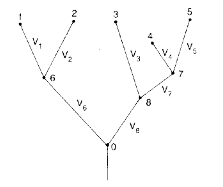
\includegraphics{media/ml.png}
  \caption{An example tree for likelihood calculation. This figure is taken from the paper written by Feslenstein 1981}
  \label{fig:ml}
\end{centering}
\end{figure}

\subsubsection*{Branch optimization}
To find a tree with the highest likelihood, we first start by maximizing the likelihood of a topology. Note that, with different branch length assignments, one topology can represent multiple different tree structures. By iteratively optimizing the length of all branches within in a topology, we can compute the Maximum Likelihood value that can be achieved by the topology (see (Felsenstein 1998) for the optimization of a single branch). Using the topology searching methods, we can then compare the Maximum Likelihood values of topologies to find a topology whose Maximum Likelihood is maximum. Then, the tree structure that gives the Maximum Likelihood value for the best topology is outputted as a resulting phylogenetic tree.

\subsubsection*{Merits and Critiques} 

While the Maximum Likelihood method might produce more accurate trees when
compared to other reconstruction methods, it is computationally costly,
mainly due to the likelihood calculations in the branch optimization
process. The big-O runtime estimation of the algorithm is $O(mn^6)$ with the progressive topology and $O(kmn^5)$ with the hill-climb approach, where $k$ is the number of hill-climb iterations, $m$ is the length of DNA sequences, and $n$ is the number of species. The Maximum Likelihood algorithm also assumes that the nucleotides mutate site-independently, and thus, it does not accurately account for changes such as insertion or deletion. Commonly accepted solutions to this indel problem are (i) remove all sites in which any gap appears, (ii) assign an imaginary nucleotide for gaps, and (iii) treat gaps as missing data. In this project, we used the option (ii), as Evans et al showed that the option (iii) can have deleterious effects on the reconstruction \cite{evansphylogenetic}.

\section*{Tree Comparison Algorithms}
In order to properly compare alignment and reconstruction methods, we require methods of comparing their ultimate outputs. We decided to use two different tree-distance metrics; one focused on absolute distance between species that utilized branch lengths, and one concerned with overall tree topology. Together, we believe these metrics summarize the differences and similarities between trees effectively. Note that these two metrics are part of a larger class of comparison methods known as ``dissimilarity metrics;'' this means that higher values indicate greater dissimilarity.

\subsection*{Quartet Distance: Topological Metric}
\begin{figure}
\begin{centering}
  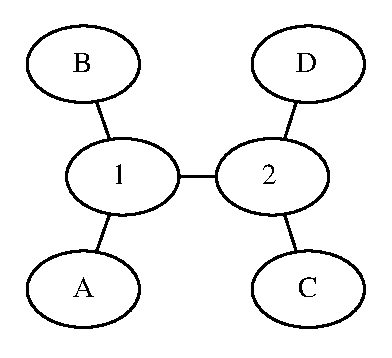
\includegraphics[width=80mm]{media/quartet.eps}
  \caption{An example of a quartet, denoted as $AB|CD$.}
  \label{fig:quartet}
\end{centering}
\end{figure}
To compare the similarity of topologies numerically, we employ a ``quartet'' based method, first proposed for this purpose by Estabrook, McMorris and Meacham \cite{estabrook1985comparison}. A quartet is a phylogenetic tree with only four species, divided by two internal nodes as in Figure ~\ref{fig:quartet}. To ``reduce'' a phylogeny to a quartet given four species, first, remove all non-desired species from the tree. Next, remove edges and internal nodes shifting your remaining species appropriately until you are left with only a quartet. This quartet should maintain some structural properties of the original tree; the remaining species now represent reductions of subtrees in their original topological formations. Computing a phylogenetic reduction is $O(n)$ because it requires a single traversal of the tree. Many previous studies have employed quartet distance as a means of analyzing the similarity of phylogenetic topologies in both theoretical an practical settings. For instance, Puigbo et al. \cite{puigbo2010tree} utilize this metric in their analysis of horizontal gene transfer in prokaryote evolution.

To compute the quartet-distance between any two topologies, say $T_1$ and $T_2$, that contain the same $n$ species, we compute all size-4 subsets $\{a,b,c,d\}$ of the $n$ species and count the number of times the reduction of $T_1$ to $\{a,b,c,d\}$ doesn't match the reduction of $T_2$ to $\{a,b,c,d\}$. The brute force algorithm, as described, is $O(n^5)$ because there exist $O(n^4)$ size-4 subsets of the $n$ species, and for each subset, two $O(n)$ reductions must be computed.

Fortunately, there exist algorithms that reduce the time complexity of this computation significantly; Brodal et al. \cite{brodal2004computing} present an $O(nlogn)$ solution to the quartet-distance problem, which represents the current state-of-the-art. For our purposes, we utilize a simpler $O(n^3)$ solution, originally proposed by Christiansen et al. \cite{christiansen2005computing}.

Central to this improved algorithm is the fact that, given any three species $\{a,b,c\}$ within a bifurcating phylogeny, there is exactly one internal node such that the paths between $\langle a, b \rangle$, $\langle b, c \rangle$, and $\langle a, c \rangle$ intersect at that node. Deleting such an internal node and its incident edges would result in three subtrees, each containing one of $a$, $b$, and $c$. Denote the subtrees as $T^a$, $T^b$, and $T^c$. For each species $x \in T^a - \{a\}$, we can determine that the quartet of our original tree restricted to $\{a,b,c,x\}$ will be $ax|bc$. Symmetric principles apply to $T^b$ and $T^c$. While further algorithmic detail is not necessary, this is the primary observation that allows us to reduce our time complexity to $O(n^3)$, as we now restrict our consideration to species subsets of size three.

\subsection*{Pairwise Path Distance: Branch Length Metric}
Because quartet distance doesn't account for branch lengths and many of our tree reconstruction algorithms produce weighted topologies, a secondary metric that accounts for this additional information is required. First proposed by Williams and Clifford \cite{williams1971comparison}, we utilize a version of pairwise pathlength distance similar to that proposed by Steel and Penny \cite{steel1993distributions}. The focus of this comparison method is computing all the pathlength between all pairs of species in a given phylogeny.

More specifically, pairwise pathlength distance can be computed as follows. Given two trees with associated branch lengths $T_1$ and $T_2$ each containing species $\{S_1, S_2 \ldots S_n\}$, consider a fixed ordering of all possible species pairs $\langle (S_1, S_2), (S_1, S_3) \ldots (S_{n-1}, S_n) \rangle$. Consider $\vec{d_1}, \vec{d_2}$, the ordered pairwise pathlength distances between the species specified in the ordering for $T_1$ and $T_2$. After normalizing these vectors such that each of their largest components is equal to one, the pairwise path distance between $T_1$ and $T_2$, then, is given by
\begin{align}
  d_{path}(T_1, T_2) = ||\vec{d_1} - \vec{d_2}||_2
\end{align}
where $||\cdot||_2$ is the $L_2$ (Euclidean) norm.

To compute pathlengths between all pairs of nodes in a weighted graph, we use the Floyd-Warshall algorithm \cite{floyd1962algorithm}, which performs the desired computation in $O(|V|^3)$ in a general graph. In our case, $O(|V|^3) = O(n^3)$, where $n$ is the number of species in a tree. This term dominates the computation of pairwise path distance, and represents the overall runtime of our approach, given two phylogenies.

\section*{Experiments}

\subsection*{Methods}
To compare our algorithms, we design two basic experiments, one for synthetic data, and one for real
data.

\subsubsection*{Synthetic Data Experiments}
Our random data generator is capable of producing testing examples $\langle T, D \rangle$ where
$T$ is a randomly generated phylogenetic tree containing $n$ species, and $D$ is a set of $n$ 
sequences generated based on that synthetic tree. We can use $D$ as input to a total of 18
combinations of the 3 multiple sequence alignment algorithms and the 6 reconstruction algorithms.
The output of these algorithms can be then be compared to the true tree $T$ and the tree
using either of our distance metrics.

Our random data generator is governed by several input parameters, including the number of desired
species, the global mutation rate, and the starting sequence length. Because of our limited computational
resources, we were only able to execute a subset of the large number of possible experiment. In total, we
completed tree reconstructions from all possible pairs of alignment and reconstruction algorithms in the
Cartesian product \{Clustal-W, Center Star\} $\times$ \{Neighbor Joining, Maximum Parsimony Progressive,
Maximum Parsimony Hill-Climbing, Maximum Likelihood Progressive, Maximum Likelihood Hill-Climbing,
MCMC with likelihood\}. MCMC was ran for 200 iterations. 

We executed each of these 12 reconstruction methods on 14 randomly generated datasets with varying number of
species. The randomly generated datasets we used had a total number of species between four and eight.
Furthermore, we have a constant mutation parameter and seed the mutation process with sequences
of length 200. This gives us five distinct datasets.

For each of the five datasets and 12 reconstruction methods, we evaluate the performance of our
algorithms over 14 trials. To evaluate their outputs, we compute the average
quartet distances and the average pairwise path distances, normalized to $[0, 1]$.
Notably, one of our reconstruction methods, MP, does not produce meaningful branch length
predictions, so for any analysis associated with MPP or MPH, we only use quartet distance.

Furthermore, we measure the average runtime of each algorithm in each scenario to quantify
the computational efficiency of each approach.

Questions we address with experiment one include\ldots
\begin{enumerate}
  \item Do different algorithms perform significantly better or worse when there are different numbers of species in the dataset?
  \item Does algorithm runtime depend on problem difficulty, rather than problem size?
\end{enumerate}

\subsubsection*{Real Data Experiments}
We have a dataset $\langle T, D \rangle$ where $T$ is the commonly accepted phylogeny
for 53 species (50 primates and 3 non-primates), and $D$ are the DNA sequences of the
mitochondrial cytochrome c oxidase 
subunit 1 (COX1) of those real species \cite{perelman2011molecular}. We decided to use the phylogeny of
great apes because it is well-studied and commonly agreed upon \cite{perelman2011molecular}. This makes the commonly accepted
ape phylogeny a great candidate for a ``ground truth'' to compare against.

COX1 is a popular choice for phylogenetic reconstruction 
because it is highly conserved due to its involvement with aerobic respiration \cite{oxidase2009electron}.
To produce varying numbers of species in our input data, we
can select random subsets of the 53 extant species for analysis.

\begin{enumerate}
  \item 14 test examples $\{\langle T, D \rangle\}$ with 5 species.
  \item 14 test examples $\{\langle T, D \rangle\}$ with 8 species.
\end{enumerate}

Due to the computational intensity of the experiments, we were only able to run Clustal-W alignments
paired with our six reconstruction method for each of these 28 datasets.

Questions we address with experiment one include\ldots
\begin{enumerate}
  \item Do the random data results match the real data results?
  \item Which algorithm performs fastest on the real data?
  \item Which algorithm produces the most accurate tree on the real data?
\end{enumerate}

\subsection*{Reconstruction Hypotheses}
We hypothesize that the method with Center Star and Neighbor Joining has the shortest average running
time on randomly generated data due to its algorithmic simplicity. We believe that Clustal W/Maximum Likelihood
and Clustal/Markov Chain Monte Carlo will perform better than other methods in terms of the accuracy of tree reconstruction
on the random data because these algorithms make fewer ``binding'' local decisions that might cause a build-up of errors.

\subsubsection*{Parallel Experiment}

We execute the sequential and parallel version of our code on 4 randomly generated datasets consisting of four, five, six and seven species, and measure the resulting speedup
on a machine with 8 processors. Of our implementations, Neighbor Joining does not assume site independence and it is consequently excluded from
our analyses. Because each algorithm's asymptotic runtime is simply multiplied by a constant factor representing genomic length in accordance
with the site independence assumption (i.e. an $O(n^2)$ computation for a single site becomes an $O(mn^2)$ computation for $m$ sites) we suspect
that speedup between our algorithms will be roughly the same, and consistent over varying numbers of species.

\subsection*{Results}

\subsubsection*{Synthetic Data Experiments}

\begin{itemize}
  \item \textbf{Pairwise Distance.} Figure \ref{8pairwiseSynthetic} illustrates the accuracy of our tree outputs in terms of pairwise distance. Notably, Neighbor Joining and Maximum Likelihood Progressive consistently did better than other reconstruction algorithms. On the other hand, the trees produced by the Markov Chain Monte Carlo method did significantly worse than trees produced by any other reconstruction method. Choice of multiple sequence alignment algorithms did not have a visible effect on the accuracy of a resulting tree. 
  \item \textbf{Quartet Distance.} The results for the quartet distance analysis is represented in Figure \ref{8quartetSynthetic}. Reconstruction with Neighbor Joining, Maximum Parsimony Progressive, and Maximum Likelihood Progressive methods outperformed other methods. Again, choice of multiple sequence alignment algorithms did not have a visible effect on the accuracy of a resulting tree. 
\end{itemize}

 \begin{sidewaysfigure*} %super janky way of displaying full page box plot table
    \vspace{0 mm}
    \hspace{-40mm}
	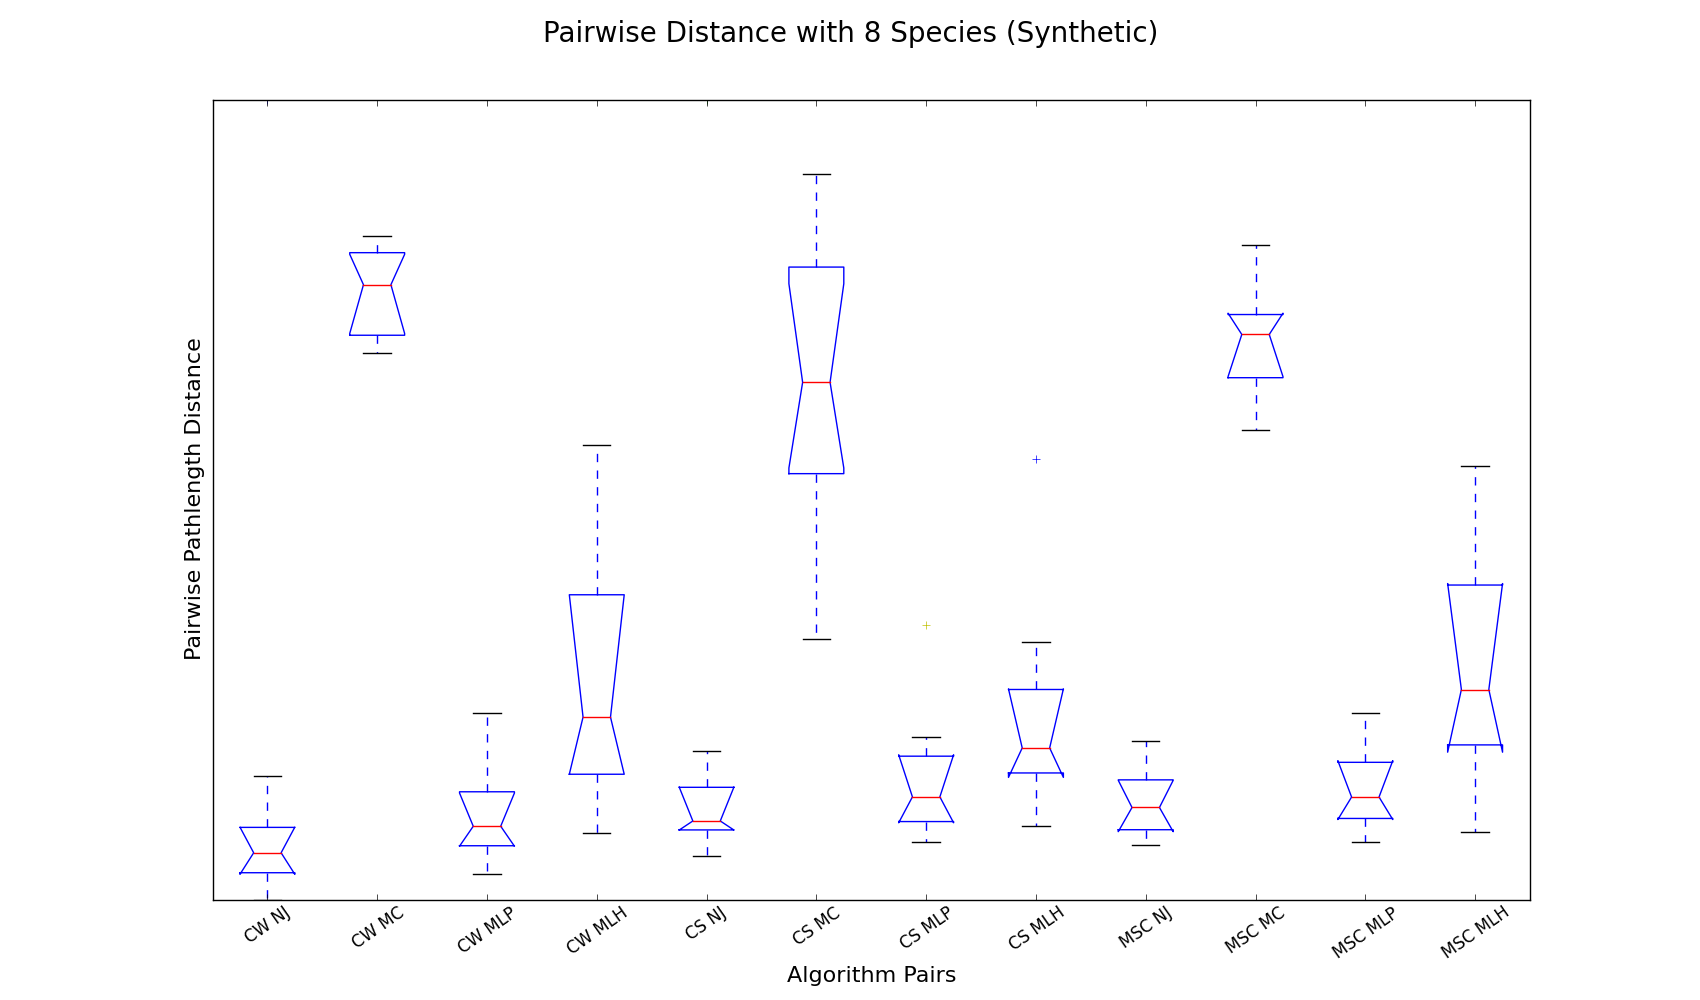
\includegraphics[scale=.72]{./media/8pairwiseSynthetic.png}
	\caption{The resulting total PPLD distance between each method's generated trees and the source tree which is assumed to be correct. Higher values are considered to be further from the original tree.} % title of Table 
	\label{8pairwiseSynthetic}

  \end{sidewaysfigure*}
  
   \begin{sidewaysfigure*} %super janky way of displaying full page box plot table
    \vspace{0 mm}
    \hspace{-37mm}
	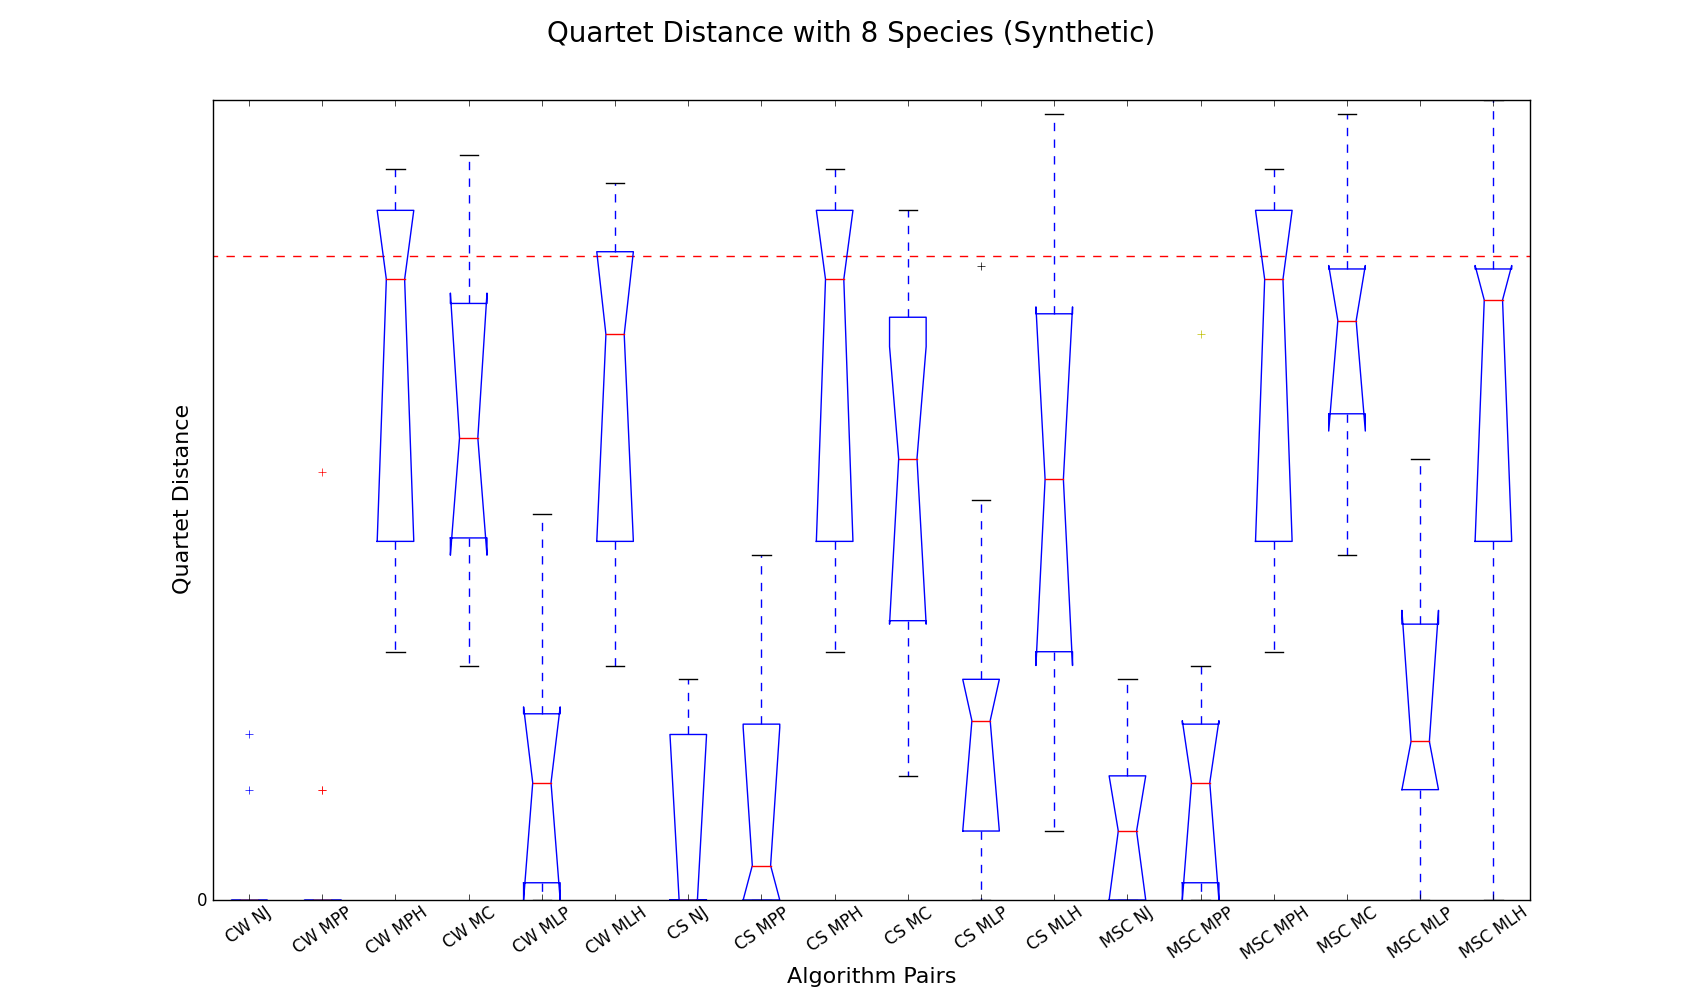
\includegraphics[scale=.72]{./media/8quartetSynthetic.png}
	\caption{The resulting total quartet distance between each method's generated trees and the source tree which is assumed to be correct. Higher values are considered to be further from the original tree. The red dotted line represents the distance between a randomly guessed tree and the original tree.} % title of Table 
	\label{8quartetSynthetic}

  \end{sidewaysfigure*}

\subsubsection*{Real Data Experiments}
Due to an unexpected bug found late in our Maximum Likelihood algorithm and the constraint of time, we were not able to obtain complete results for the real data experiments. However, experiments are running in progress and results will be available soon.

\subsubsection*{Parallel Experiment}

Results from our parallel tests are illustrated in Figure \ref{paralleltime}. Clearly, our results were not consistent with our hypothesis; speedup deviated significantly from the theoretical 7-8x for all algorithms. This is an indication that parallel theory does not always align with parallel implementation and significant care must be taken to achieve optimal performance.

The speedup of MLH and MLP were fairly consistent over different numbers of species, but only a 3x speedup was achieved. MPH and MPP were no faster (and sometimes slower) than their sequential counterparts; this is likely a result of their relatively low runtimes. In these cases and at this scale, the overhead associated with creating threads counteracted the parallel speedup attained.

Most interesting were our speedup results for MCMC. Here, speedup decreased significantly as the number of species increased. Because MCMC is parallelized in the same way as MLH and MLP (all three methods use a parallel version of the likelihood computation) this result was particularly unexpected.

\begin{figure}[ht!]
\begin{centering}
  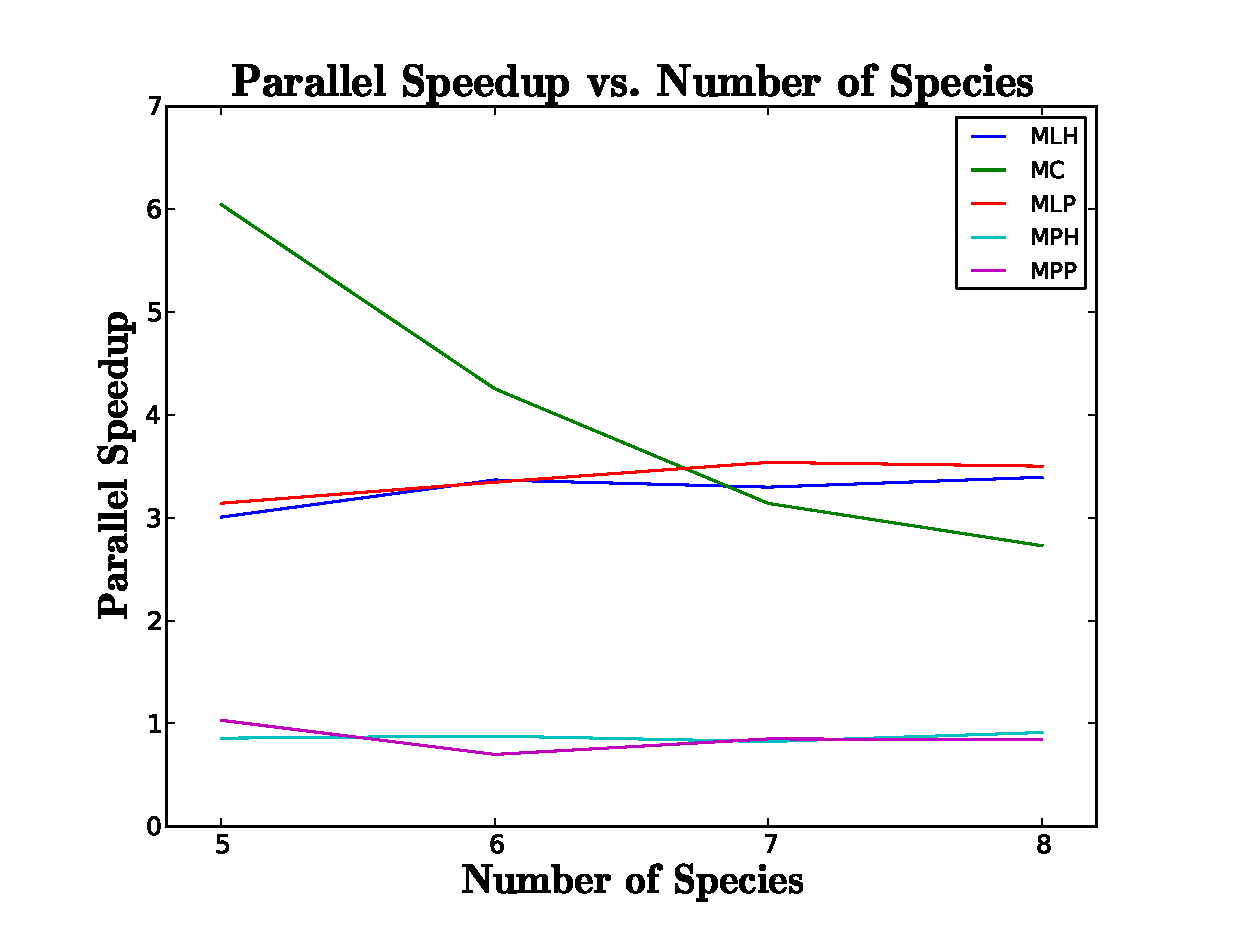
\includegraphics[scale=.45]{media/para.eps}
  \caption{Parallel speedup of our implementations on several test synthetic datasets (bp = 200) of varying size on a machine with 8 processors. We allowed OpenMP to use 64 threads.}
  \label{paralleltime}
\end{centering}
\end{figure}


\begin{figure}[ht!]
\begin{centering}
  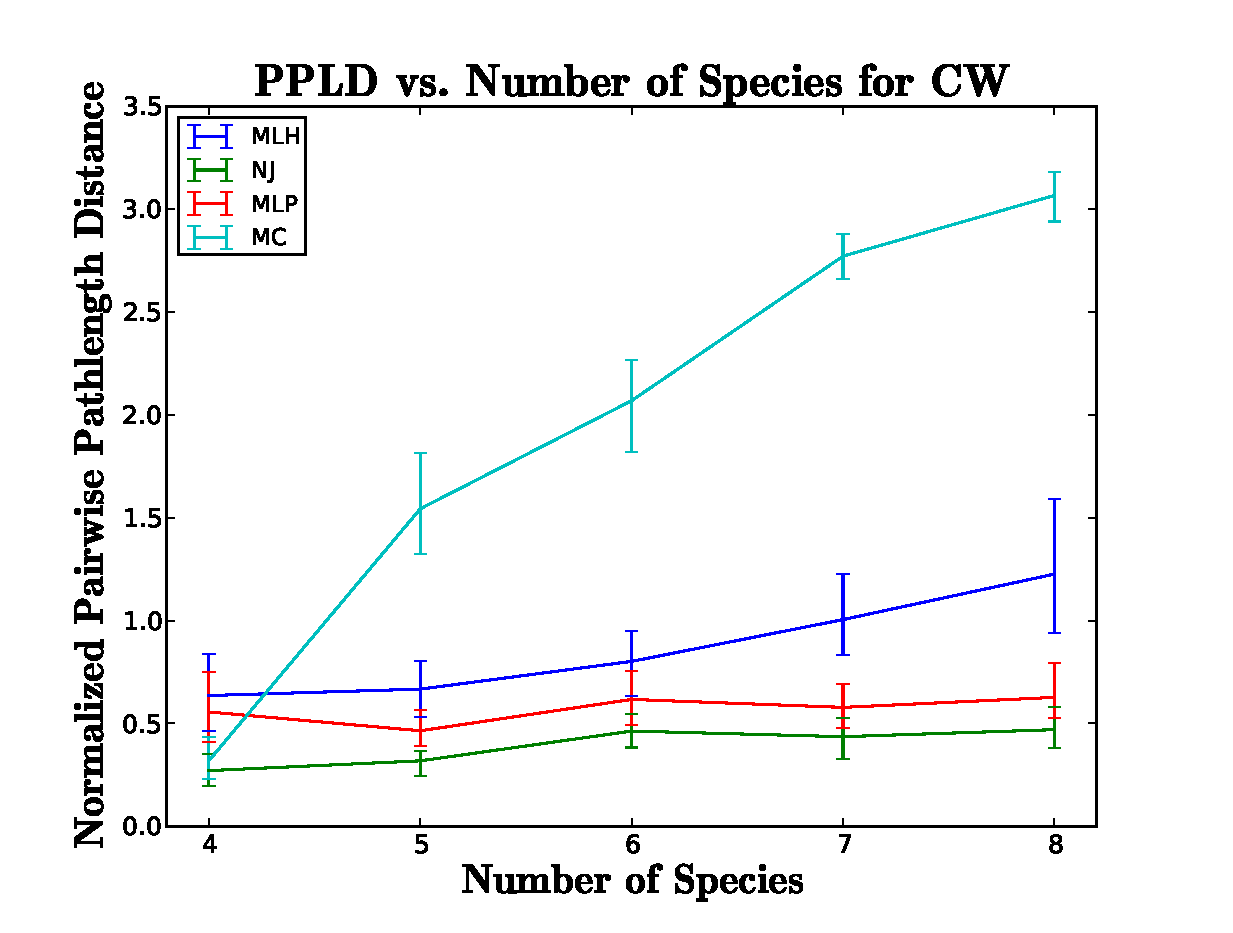
\includegraphics[scale=.45]{media/accGraphs/CWacc.eps}
  \caption{Pairwise pathlength distance of several methods over varying numbers of species. Results indicate that MCMC and MLH might become relatively less accurate as the input size increases.}
  \label{accuracynumspec}
\end{centering}
\end{figure}
\subsubsection*{Running Time}

Runtime analysis of both synthetic (Figure \ref{synthetictime}) and real data (Figure \ref{realtime}) suggests the following:
\begin{enumerate}
\item Neighbor Joining gave the fastest performance.
\item Maximum Likelihood performed worse than Maximum Parsimony.
\item Monte Carlo Markov Chain performed slower than Maximum Likelihood for smaller synthetic data sets, and faster than Maximum Likelihood hill-climbing for bigger synthetic data sets.
\end{enumerate}
These results are similar when using Center Star and MUSCLE alignment algorithms.
\begin{figure}[ht!]
\begin{centering}
  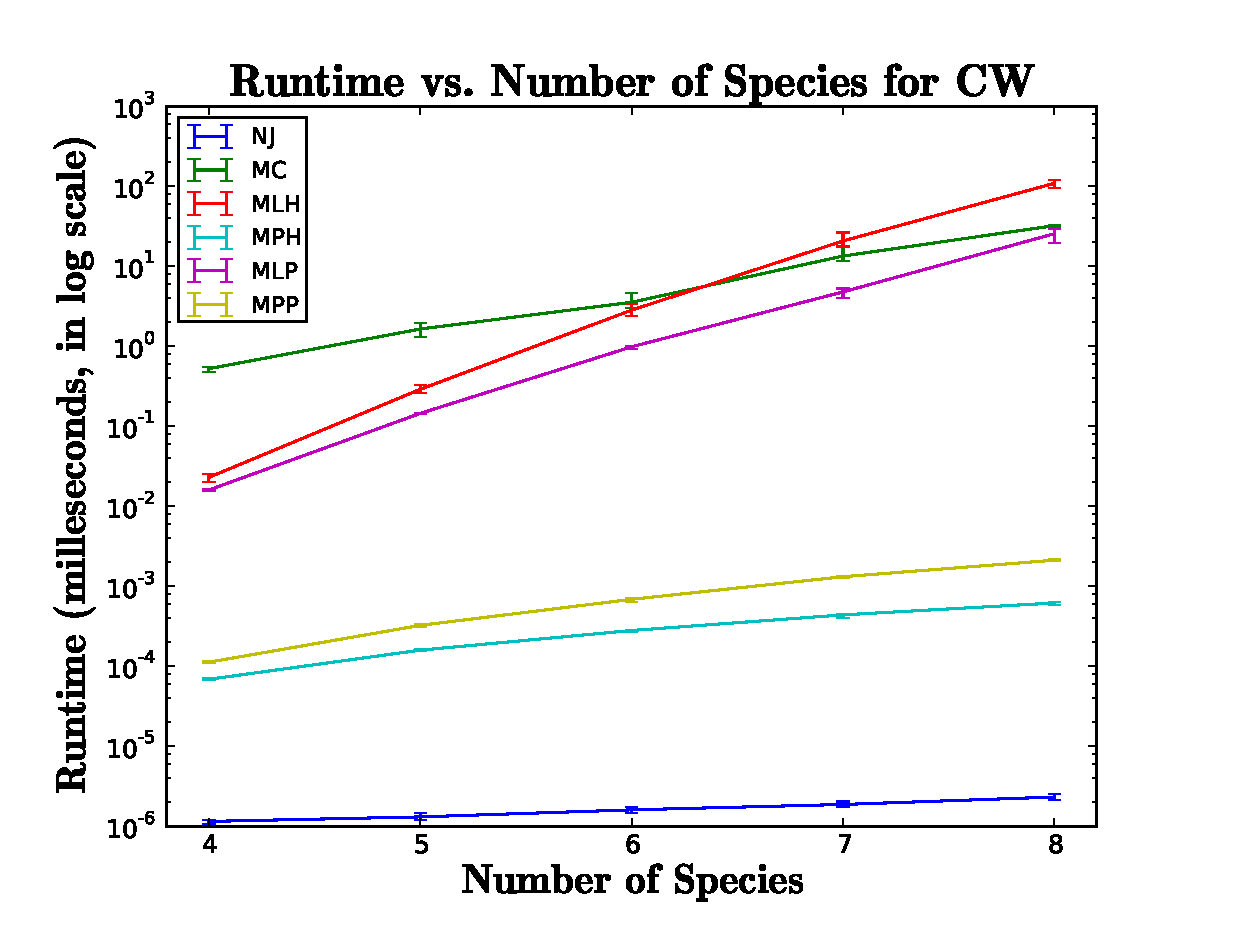
\includegraphics[scale=.45]{media/runtimeGraphs/CW.eps}
  \caption{Runtime comparison of reconstruction algorithms on synthetic data sets using Clustal-W as our alignment algorithm.}
  \label{synthetictime}
\end{centering}
\end{figure}

\begin{figure}[ht!]
\begin{centering}
  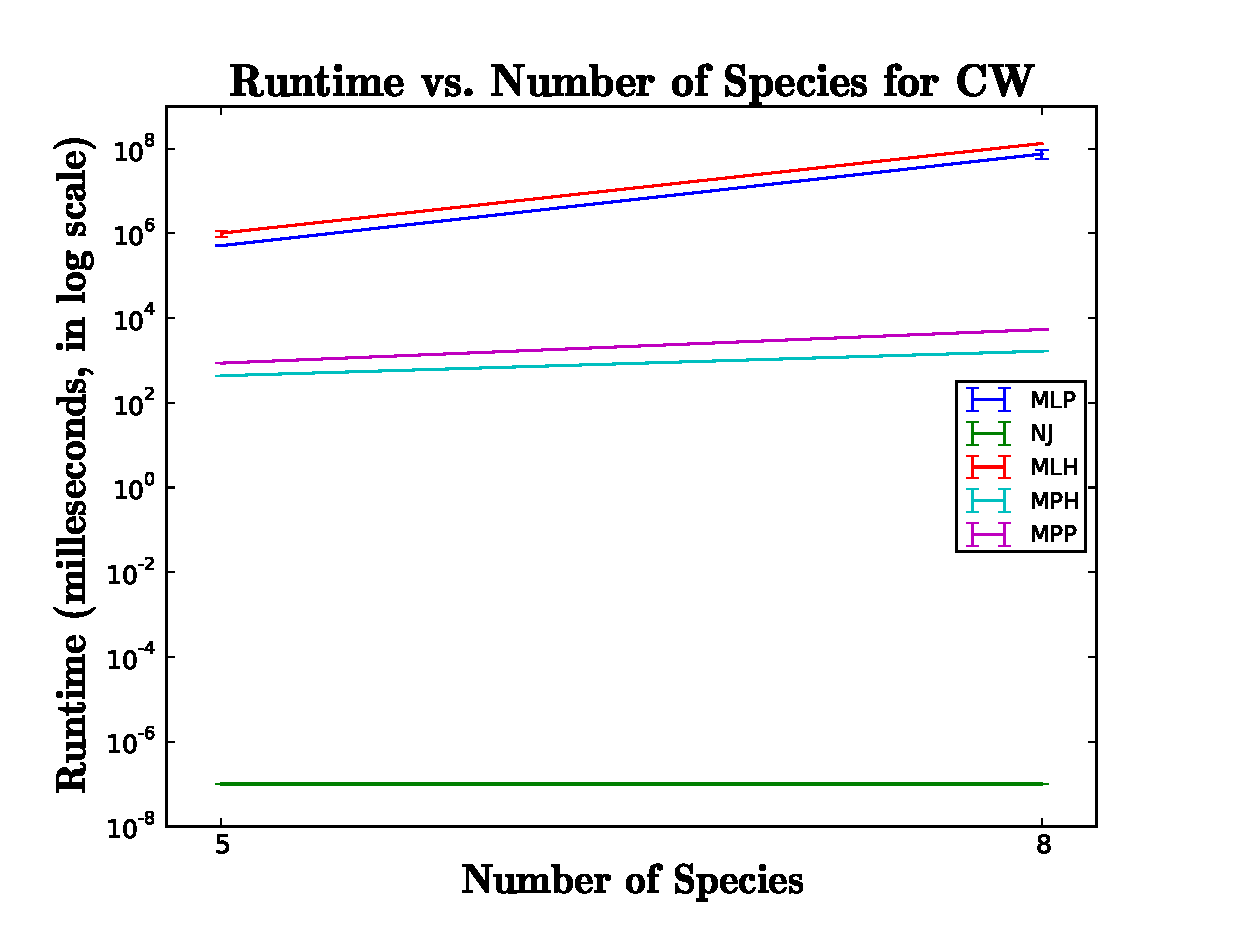
\includegraphics[scale=.45]{media/runtimeGraphs/CWreal.eps}
  \caption{Runtime comparison of reconstruction algorithms on real data sets using Clustal-W as our alignment algorithm.}
  \label{realtime}
\end{centering}
\end{figure}


\subsection*{Discussion}
\subsubsection*{Tree Accuracy}
In terms of pairwise distance metric, ML Progressive outperformed ML Hill-climb. The only difference between the two reconstruction algorithms was their topology searching method: progressive vs. hill-climb approach. The difference in performance between these two algorithms can be explained as follows. The downside of the progressive approach is that it makes local decisions when searching through the space of possible topologies, and thus, a resulting tree topology can sometimes be unreliable. However, this does not have a big impact when trees are evaluated on pairwise distance, because it only measures the distances between pairs of leaf nodes; pairwise distance does not account for the position of a node within a tree. On the other hand, the hillclimb approach can sometime gets caught in a local optimum. In our case, it is likely that the downside of the hillclimb approach had a larger impact on resulting trees. 

For quartet distance metric, Maximum Parsimony also achieved results with equally high accuracies as NJ and ML methods. This is in agreement with \cite{kuhner1994simulation}, which suggests that under low nucleotide substitution rates, NJ, MP, and ML should be equally successful. 
Hill-climbing approaches performed significantly worse than progressive approaches in terms of quartet distance metric. Again, this is likely due to the fact that hill-climbing approaches can sometimes only find the local optimal topology rather than the true global optimum.

NJ produced accurate results in our study for both pairwise distance and quartet distance. This was in accordance with \cite{saitou1989relative}, which suggested that NJ performs slightly better than ML methods under constant nucleotide substitution rates.

MCMC performed significantly worse than other reconstruction algorithms in terms of both quartet and pairwise distance metrics. This is likely because we did not run the algorithm long enough to find a reasonable global optimum. In order to find trees close to the global optimum in our sample space, the suggested number of iterations was 2000 \cite{larget1999markov}. Due to the time constraints in our project, we only ran 200 iterations.

In Figure \ref{accuracynumspec}, we compare the correctness of tree output of various algorithms when problems increase in size. Notably MCMC becomes increasingly less accurate when the number of species increases. This is likely a reflection of the fact that tree space is less able to be explored in a fixed 200 iterations when more species are added. Furthermore, using likelihood and hill climbing appears to become less correct and more variable for larger problems as well. Because the objective function increases significantly in complexity as the number of species increases, it's likely the case that getting caught in local optima becomes increasingly common. On the other hand, NJ and MLP perform relatively consistently, indicating their potential accuracy on larger datasets.

\subsubsection*{Running Time}
The expected efficiency of NJ is consistent with our experimental results. ML, on the other hand, is considered computationally costly with progressive topology ($O(mn^6)$) and with the hill-climb approach ($O(kmn^5)$) due to the branch optimization process. MCMC, which uses ML's likelihood calculations, is also computationally expensive. These theoretical observations also agree with our experimental results. MP had a performance speed that fell in between NJ and ML, which also fits our expectation.

\subsubsection*{Parallelization}
Our parallelization results were promising but highly inconsistent. The main downside of our consideration was its relative simplicity; parallelizing in accordance with the site independence assumption is a good place to start, but it is only a first step. Many other aspects of these algorithms, such as recursive tree traversals, can be easily and completely parallelized, and it would be exciting to pursue new avenues of optimization, particularly on specialized hardware (MapReduce clusters, GPGPUs) in future work.

The results for MCMC, where speedup decreased with increasing input size, were among the most intriguing in our entire study. Perhaps, in this case, the sequential version of this algorithm benefits from some under-the-hood compiler optimization that the other likelihood-based methods (MLH, MLP) do not.

In total, our investigation of parallelism in phylogenetic reconstruction is a small first step towards understanding the complexity involved in this rich field of optimization.

\subsection*{Conclusion}
Based on our experiments with both synthetic and real data, and our analysis of both run-time efficiencies and the accuracies of our algorithms, we conclude that for data sets with similar properties to those of our data (i.e. short sequences, low and constant nucleotide substitution rates), Neighbor Joining should be used in order to achieve the best efficiency and accurate results. Maximum Likelihood with progressive tree search creates equally accurate trees, but is far more computationally expensive.

However, due to the complexity of the real-world data sets and their varying characteristics, algorithms should be carefully chosen in order to obtain accurate results. Based on our results, we cannot determine the total superiority of a specific reconstruction method. In addition, there is no guarantee that the details of our implementation match those in the literature we surveyed. Nonetheless, our study provides a comparative approach that future research alike can undertake.

In the future, we would like to examine more types of synthetic data (perhaps varying mutation characteristics) and optimize our implementations in accordance with modern advancements to get a better sense of the current state of the field.

\subsection*{Acknowledgments}

First and foremost, we would like to acknowledge Sherri Goings for her continued advising and support throughout this project. We also thank Robert Dobrow for his assistance with Markov Chain Monte Carlo and Mike Tie for maintaining our computational resources.

\bibliographystyle{abbrv}
\bibliography{refs}
\end{document}
